\documentclass{beamer} 
\usepackage{amsmath,amsthm}
\usepackage{graphicx,microtype,parskip}
\usepackage{caption,subcaption,multirow}
\usepackage{attrib}

\frenchspacing

\usetheme{default}
\usecolortheme{whale}

\setbeamertemplate{navigation symbols}{}

\setbeamercolor{title}{fg=blue,bg=white}

\setbeamercolor{block title}{fg=white,bg=gray}
\setbeamercolor{block body}{fg=black,bg=lightgray}

\setbeamercolor{block title alerted}{fg=white,bg=darkgray}
\setbeamercolor{block body alerted}{fg=black,bg=lightgray}

%\AtBeginSection[]
%{
%  \begin{frame}
%    \tableofcontents[currentsection]
%  \end{frame}
%}

\title{Cenozoic mammals and the biology of extinction}
\author{Peter D Smits}
\institute{Committee on Evolutionary Biology, University of Chicago}

\begin{document}

\begin{frame}
  \maketitle
\end{frame}

\begin{frame}
  \frametitle{Extinction}
  \begin{quotation}
    All species that have ever lived are, to a first approximation, dead.

    \tiny{\attrib{Raup 1986 \underline{The Nemesis Affair}}}
  \end{quotation}
\end{frame}

\begin{frame}
  \frametitle{Foundation}
  \begin{alertblock}{Question}
    Why do certain taxa go extinct while others do not?
  \end{alertblock}
\end{frame}

\begin{frame}
  \frametitle{In context of this study}
  \begin{block}{Rephrased}
    How does a taxon's \alert{adaptive zone} affect \alert{extinction risk?}
  \end{block}
\end{frame}

\begin{frame}
  \frametitle{Modes of extinction}

  \hspace{\stretch{0.4}} Field of Bullets 
  \hspace{\stretch{0.5}} \textbf{--} 
  \hspace{\stretch{0.5}} Wanton 
  \hspace{\stretch{0.5}} \textbf{--} 
  \hspace{\stretch{0.5}} Fair Game 
  \hspace{\stretch{1}}

  \bigskip

  \tiny{\attrib{Raup 1991 \underline{Extinction: Bad Genes or Bad Luck?}}}

\end{frame}

\begin{frame}
  \frametitle{Van Valen's observation}

  \begin{center}
    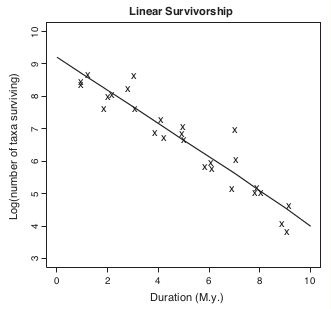
\includegraphics[height = 0.7\textheight, keepaspectratio = true]{figure/liow}

    \tiny{\attrib{Liow et al. 2011 \textit{TREE}}}
  \end{center}
\end{frame}

\begin{frame}
  \frametitle{Law of Constant Extinction}

  \begin{definition}
    Extinction rate, in a given adaptive zone, is taxon--age independent.

    \tiny{\attrib{Van Valen 1973 \textit{Evol. Theory}}}
  \end{definition}
\end{frame}

\begin{frame}
  \frametitle{Biology and extinction}

  \begin{block}{Questions}
    \begin{itemize}
      \item Do interactions involved in environmental preference predict differential survival?
        \begin{itemize}
          \item Is survival best modeled by a single interactor or multiple interactors? 
          \item How do factors, such as climate, contribute? 
        \end{itemize}
      \item Is extinction taxon-age independent or dependent?
      \item Do genera and species have fundamentally different survival distributions?
    \end{itemize}
  \end{block}
\end{frame}

\begin{frame}
  \frametitle{Survival analysis}

  \begin{definition}
    Analysis of \alert{time till event data}.

    i.e. Time from origination to extinction (\textbf{duration, \(T\)}).
  \end{definition}

\end{frame}

\begin{frame}
  \frametitle{Formalization of Van Valen}

  \begin{block}{Law of Constant Extinction}
    \begin{center}
      \begin{tabular}{@{}l@{}}\(T \sim Exp(\lambda)\)\end{tabular}
      \hspace{1.5cm}
      \begin{tabular}{@{}l@{}}\(T\): survival time\\\(\lambda\): expected number of \\extinctions per unit time\end{tabular}
    \end{center}
  \end{block}
\end{frame}

\begin{frame}
  \frametitle{Mammals}
  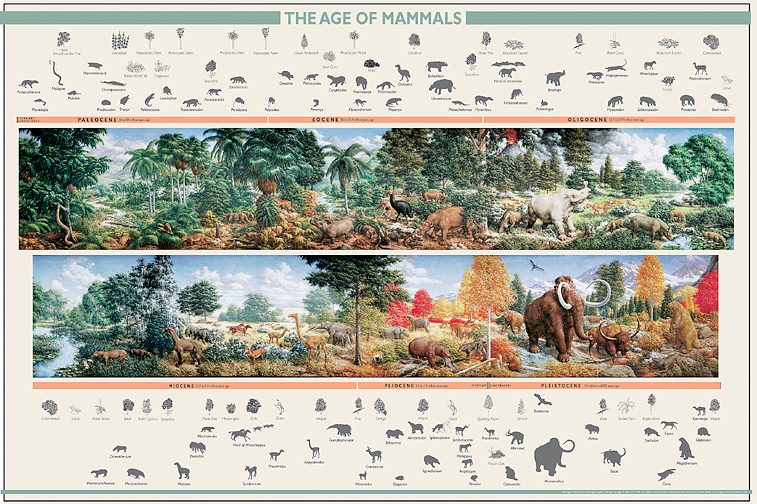
\includegraphics[height = 0.9\textheight, width = \textwidth, keepaspectratio = true]{figure/aom}

  \tiny{\attrib{Yale Peabody Museum}}
\end{frame}

\begin{frame}
  \frametitle{Regions}
  \begin{columns}
    \begin{column}{0.5\textwidth}
      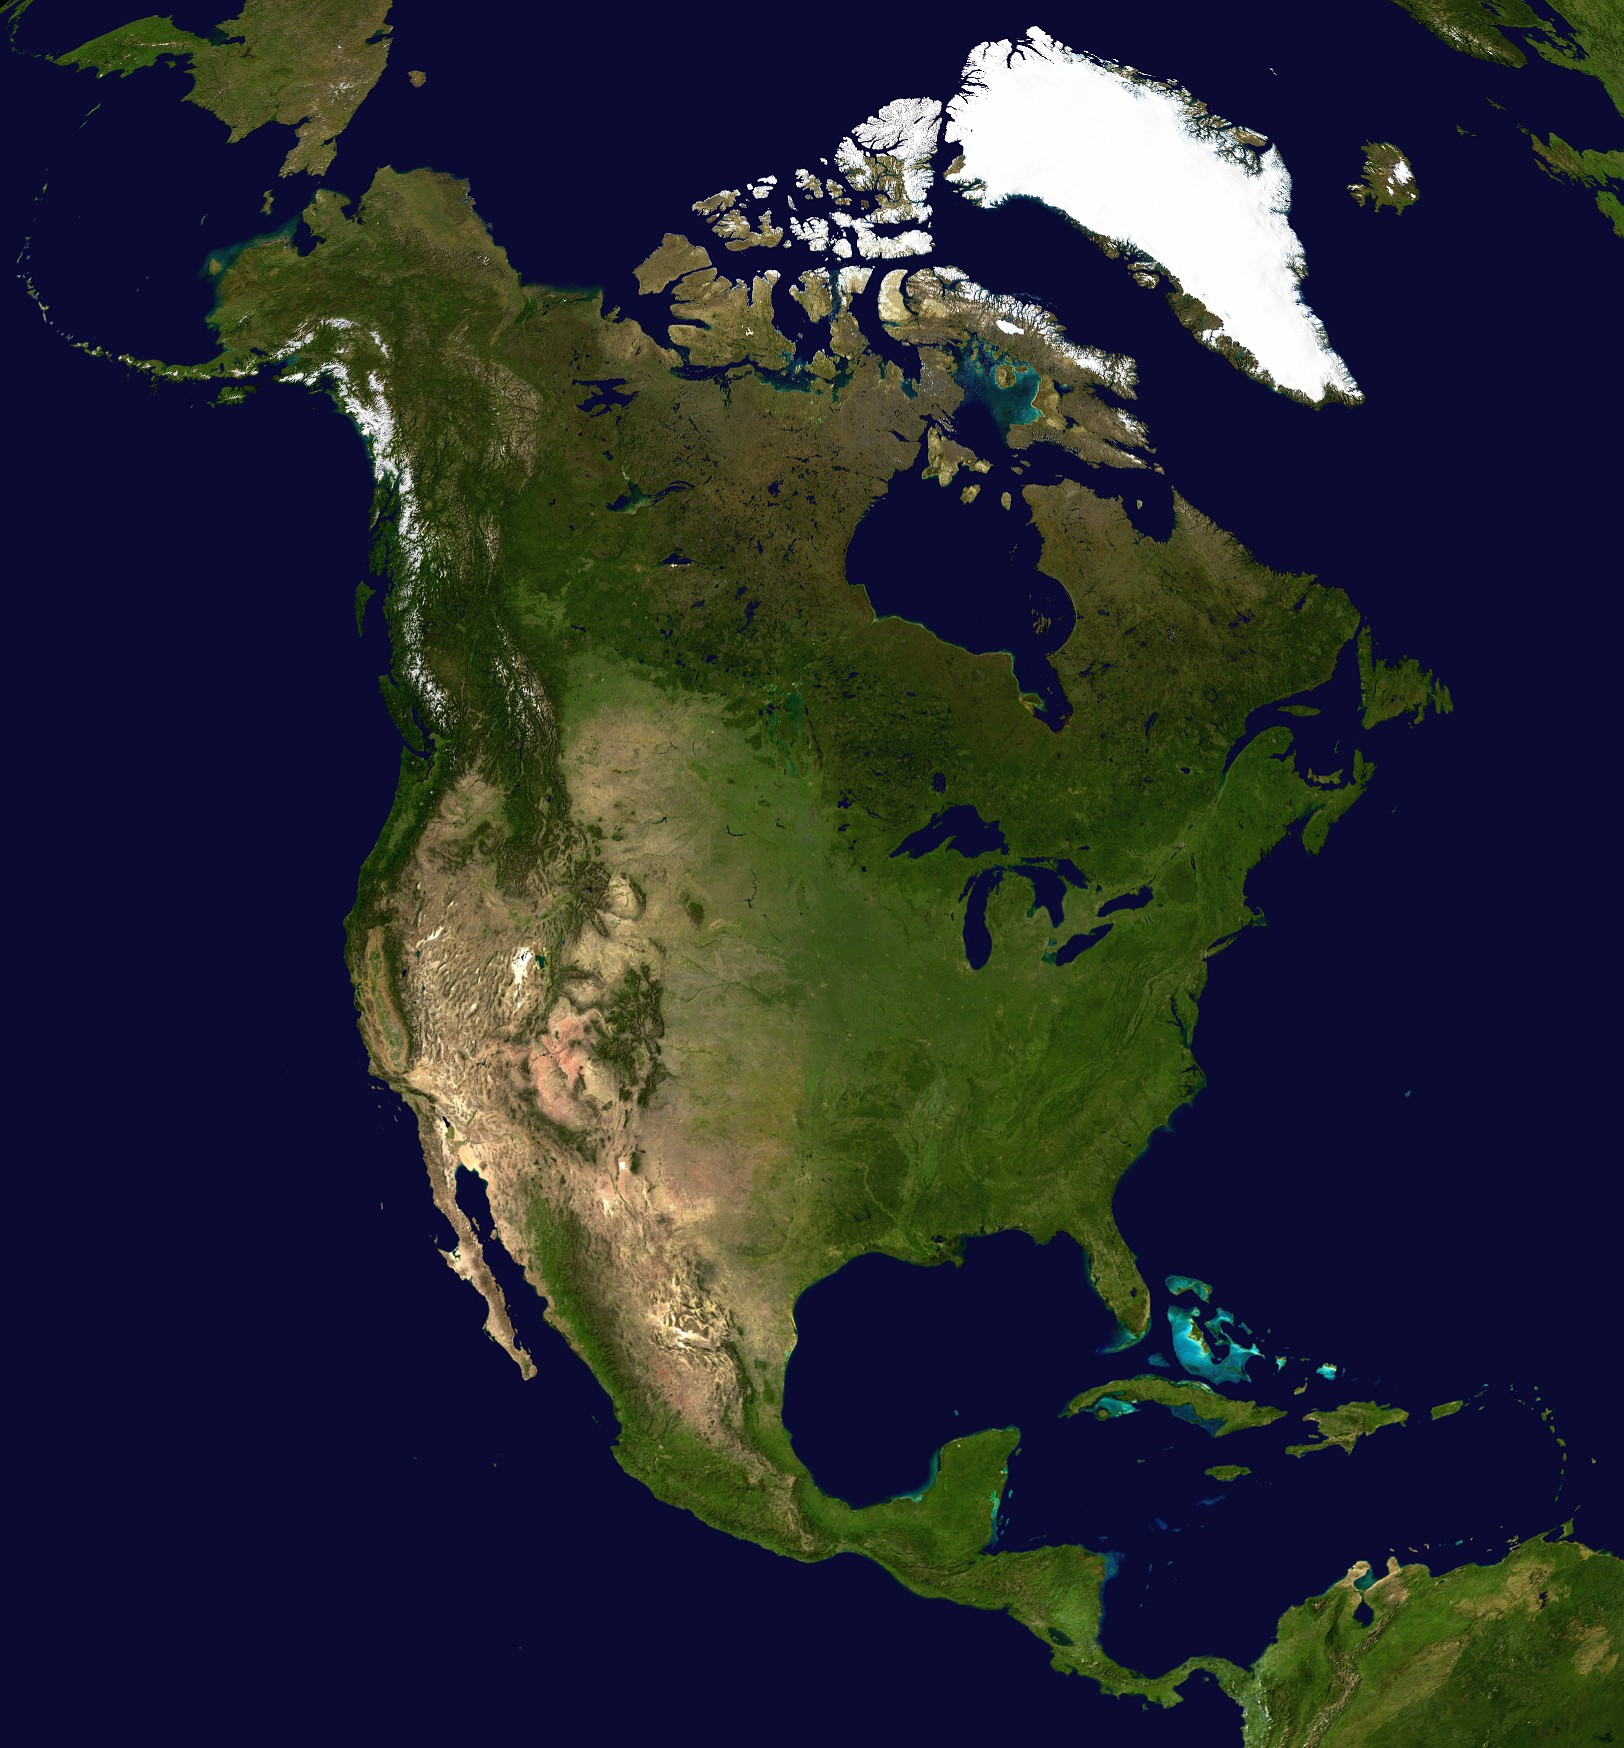
\includegraphics[height=0.5\textheight,width=\textwidth,keepaspectratio=true]{figure/na_map}
    \end{column}
    \begin{column}{0.5\textwidth}
      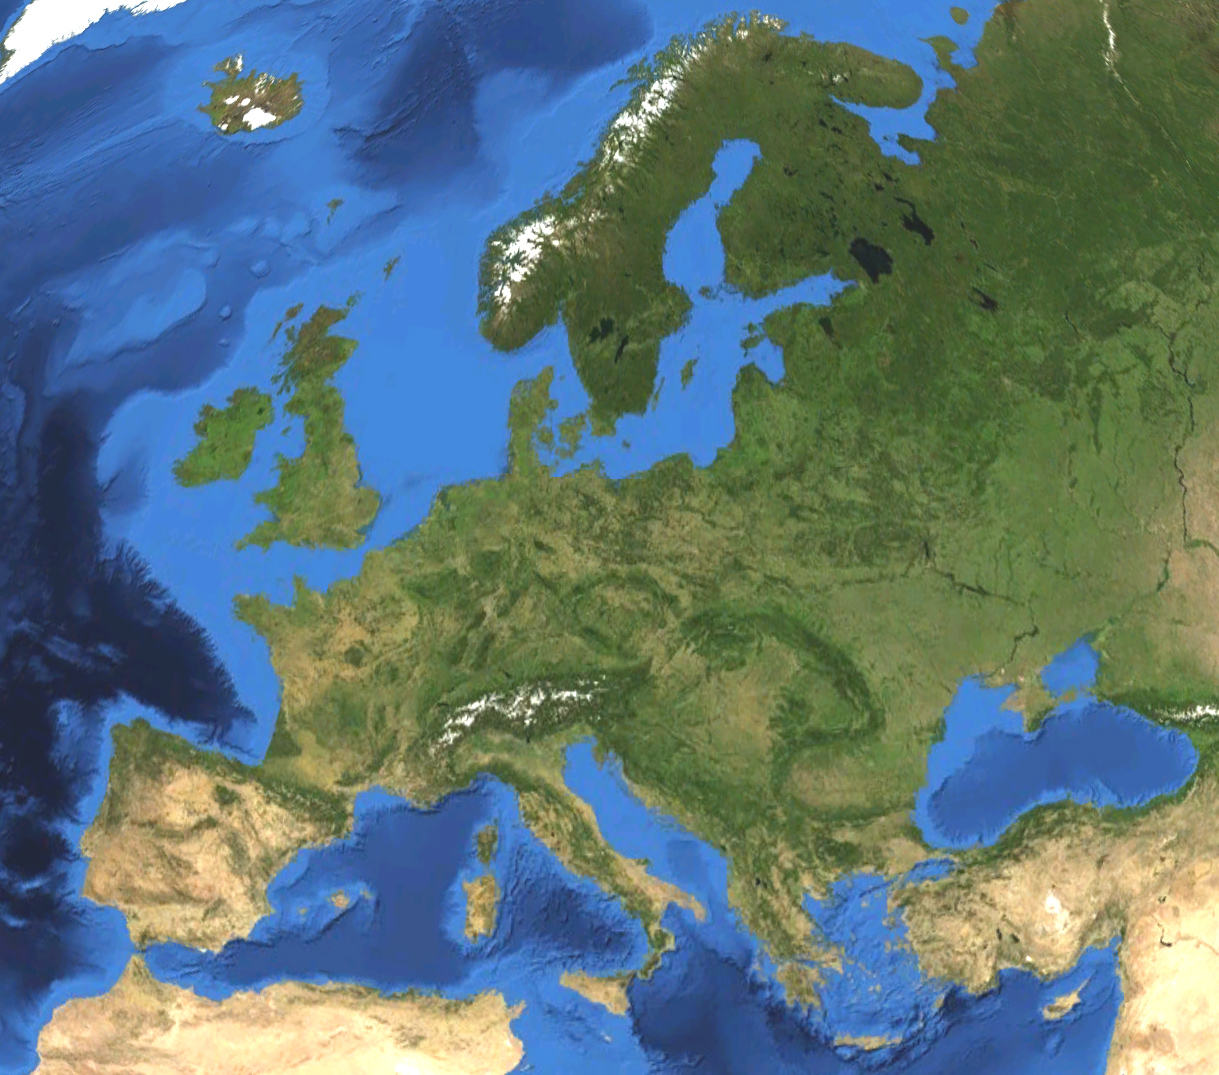
\includegraphics[height=0.7\textheight,width=\textwidth,keepaspectratio=true]{figure/euro}
    \end{column}
  \end{columns}

  \vspace{0.2cm}

  \begin{columns}
    \begin{column}{0.5\textwidth}
      North America: \\2366 species, 1003 genera 
    \end{column}
    \begin{column}{0.5\textwidth}
      Europe: \\1767 species, 658 genera
    \end{column}
  \end{columns}

\end{frame}

\begin{frame}
  \frametitle{Diet}

  \begin{columns}
    \begin{column}{0.5\textwidth}
      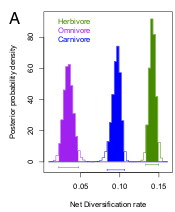
\includegraphics[height=0.5\textheight,width=\textwidth,keepaspectratio=true]{figure/dietdiv}

    \end{column}
    \begin{column}{0.5\textwidth}
      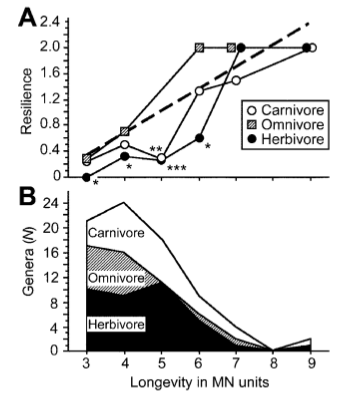
\includegraphics[height=0.5\textheight,width=\textwidth,keepaspectratio=true]{figure/jernvall}
    \end{column}
  \end{columns}

  \begin{center}
      carnivore, herbivore, omnivore, insectivore
      
      \vspace{0.2cm}

      herbivore \(>\) carnivore \hspace{0.3cm} omnivore \(\simeq\) carnivore \hspace{0.5cm} insectivore ?

    \end{center}
\end{frame}

\begin{frame}
  \frametitle{Locomotion}
  \begin{columns}
    \begin{column}{0.5\textwidth}
    \end{column}
    \begin{column}{0.5\textwidth}
      ground dwelling, scansorial, arboreal

      \vspace{0.3cm}

      \begin{itemize}
        \item ground dwelling \(>\) arboreal
          \vspace{0.2cm}
        \item scansorial \(\simeq\) ground dwelling 
      \end{itemize}
    \end{column}
  \end{columns}
\end{frame}

\begin{frame}
  \frametitle{Body size}
  \begin{columns}
    \begin{column}{0.5\textwidth}
      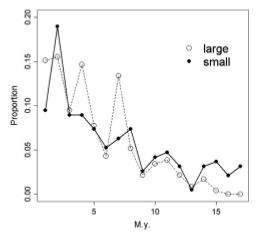
\includegraphics[height=0.4\textheight,width=\textwidth,keepaspectratio=true]{figure/liowmam}

      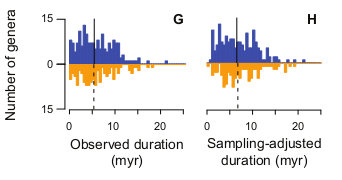
\includegraphics[height=0.4\textheight,width=\textwidth,keepaspectratio=true]{figure/susumu}
    \end{column}
    \begin{column}{0.5\textwidth}
      \(\uparrow\) mass, \(\uparrow\) range size, \(\uparrow\) survival

      \vspace{0.3cm}

      \textbf{OR}

      \vspace{0.3cm}

      \(\uparrow\) mass, \(\downarrow\) reproductive rate, \(\downarrow\) survival

    \end{column}
  \end{columns}
\end{frame}

\begin{frame}
  \frametitle{The Elephant in the Range}

  % some kind of image 

  mean, CV occupancy

  \(\uparrow\) occupancy, \(\uparrow\) duration

\end{frame}

\begin{frame}
  \frametitle{Climate}

  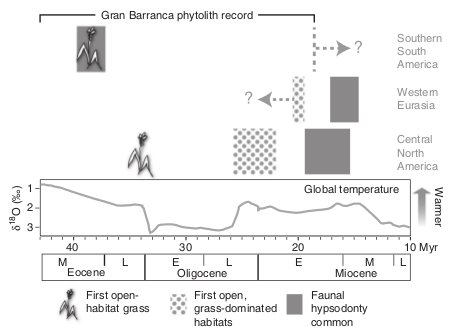
\includegraphics[height=0.8\textheight,width=\textwidth,keepaspectratio=true]{figure/stromberg}

  \tiny{\attrib{Str\"{o}mberg \textit{et al.} 2013 \textit{Nature Com.}}}
  % mean, CV, abs(diff)
\end{frame}

% plot the ``raw'' data?

\begin{frame}
  \frametitle{Model selection}
  % parameter ``importance'' as sum of weights
  % best model

\end{frame}

\begin{frame}
  \frametitle{``Best'' model}

\end{frame}

\begin{frame}
  \frametitle{Parameter interpretations}

\end{frame}

\begin{frame}
  \frametitle{Conclusions, future work}

\end{frame}

\begin{frame}
  \frametitle{Acknowledgements}
  \begin{columns}
    \begin{column}{0.5\textwidth}
      \begin{itemize}
        \item \textbf{Committee}
          \begin{itemize}
            \item Kenneth D. Angielczyk (co-advisor)
            \item Michael J. Foote (co-advisor)
            \item P. David Polly
            \item Richard H. Ree
          \end{itemize}
        \item Discussion
          \begin{itemize}
            \item David Bapst, Megan Boatright, Ben Frable, Colin Kyle, Darcy Ross, Liz Sander
            \item John Alroy, Graeme Lloyd, Kathleen Ritterbush, Carl Simpson, Graham Slater
          \end{itemize}
      \end{itemize}
    \end{column}
    \begin{column}{0.5\textwidth}
      
\includegraphics[height = 0.3\textheight, keepaspectratio = true]{figure/chicago} 
      
\includegraphics[width = 0.4\textwidth, keepaspectratio = true]{figure/field}

      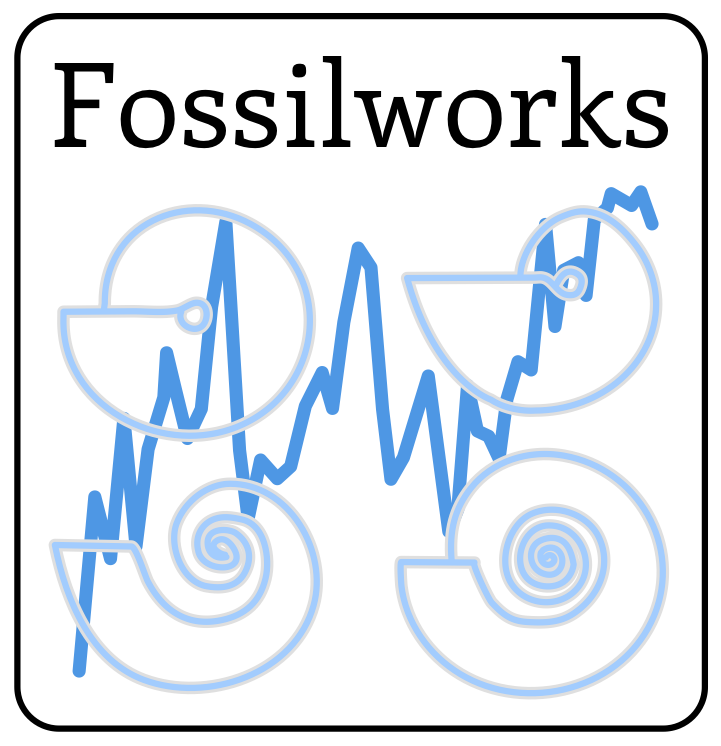
\includegraphics[height = 0.3\textheight, width = 0.5\textwidth, keepaspectratio = true]{figure/fossilworks}
      
\includegraphics[width = 0.5\textwidth, keepaspectratio = true]{figure/paleodb}

      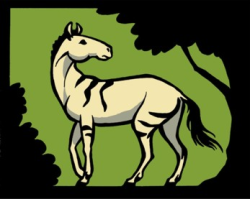
\includegraphics[height = 0.3\textheight, width = 0.5\textwidth, keepaspectratio = true]{figure/now}
    \end{column}
  \end{columns}
\end{frame}

\appendix

\begin{frame}
  \frametitle{(Informal) phylogeny}
  \begin{center}
    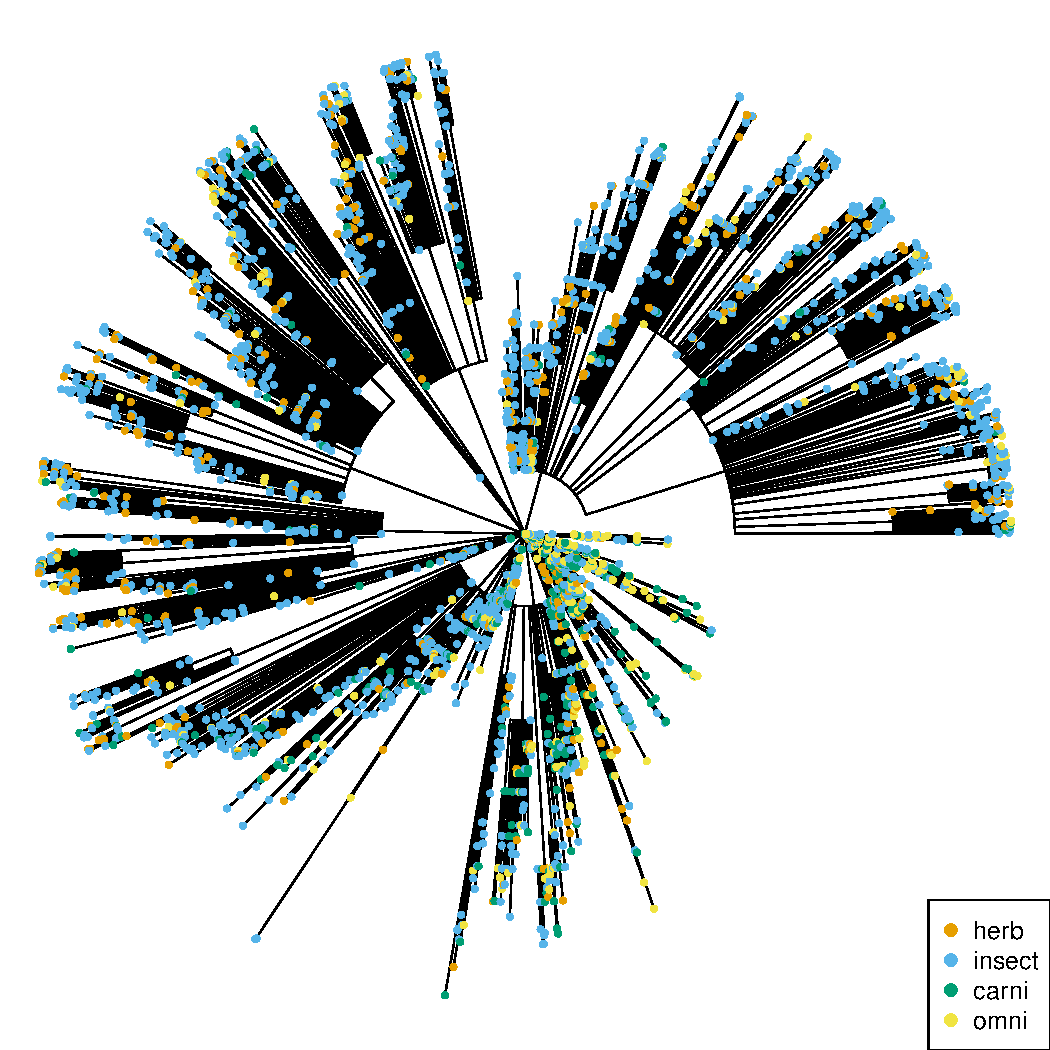
\includegraphics[height = 0.8\textheight, width = \textwidth,  keepaspectratio = true]{figure/na_phylo_diet}
  \end{center}
\end{frame}

\begin{frame}
  \frametitle{Analytical approach}

  frailty coefficient 

  conditional autoregressive prior
\end{frame}

\begin{frame}
  \frametitle{Differential preservation and survival}

  \begin{columns}
    \begin{column}{0.5\textwidth}
      \begin{center}
        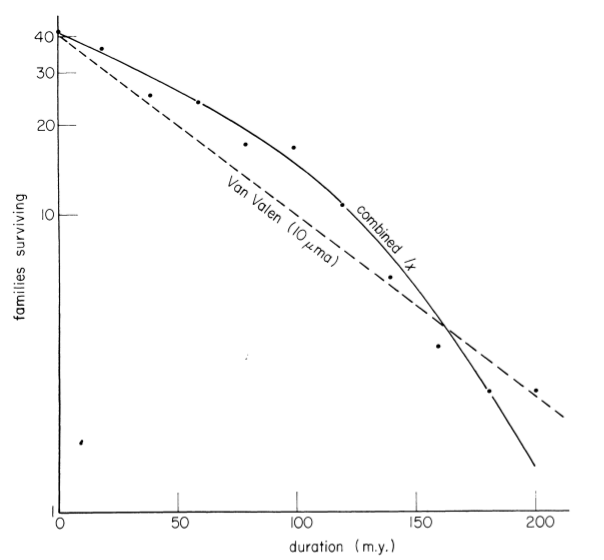
\includegraphics[height = 0.4\textheight, width = \textwidth, keepaspectratio = true]{figure/raup}

        \tiny{\attrib{Raup 1975 \textit{Paleobio.}}}

        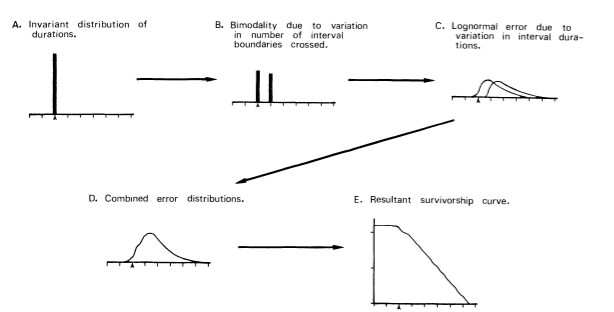
\includegraphics[height = 0.4\textheight, width = \textwidth, keepaspectratio = true]{figure/sepkoski}

        \tiny{\attrib{Sepkoski 1975 \textit{Paleobio.}}}
      \end{center}
    \end{column}
    \begin{column}{0.5\textwidth}
      two groups in four scenarios
      \begin{itemize}
        \item \(=\) birth, death; \\\(=\)preservation
        \item \(=\) birth, death; \\\(!=\)preservation
        \item \(!=\) birth, death; \\\(=\) preservation
        \item \(!=\) birth, death; \\\(!=\)preservation
      \end{itemize}
    \end{column}
  \end{columns}
\end{frame}

% any preliminary results?

\end{document}
